In this section, we report our simulation results and evaluate the
efficiency of DFDI, our program allocation algorithm, and point-based
and index-based skyline computation algorithms discussed in previous
sections of this paper. Our simulations are implemented in C\# with
.NET Framework 4 and backward compatible with .NET Framework 2.

We generated our synthetic data-sets for our simulation. Each data record
is contains $n$ attributes or an $n$-dimensional point. Our data generator
is able to generate three kinds of data-sets:
\begin{itemize}
\item Uniformed: data uniformly distributed in the data space of each
    attribute.
\item Rising: the attributes of the records are correlated to the first
    attribute of the data-set.
\item Falling: the attributes of the records are inversely correlated to
    the first attribute of the data-set.
\end{itemize}

Each data-set is characterized by the following two additional parameters:
\begin{itemize}
\item Record count: the number of records in a data-set.
\item Dimension: the number of attributes of the data-set.
\end{itemize}

The records count for our data-sets ranges from 20,000 to 100,000 and the
dimension ranges from 2 to 10 dimension. Each data-set is a file on disk
and are loaded into memory during simulation.

Our simulations are memory-based. Since this paper is the first on the topic
of using R-Tree for broadcast skyline evaluation, memory-based simulations
give us a quick tool to verify our approach since they are faster than
disk-based implementations.  The simulations load the
data-sets from disk and runs all simulations from memory.
We implemented our own in-memory R-Tree index to facilitate our simulations.
Table~\ref{tab:sim_size} lists the size matrix that is used in the
implementation of the simulation of tuning time and index percentage.

\begin{table}[h]
\caption{Simulation Size Matrix} \label{tab:sim_size}
\centering
\begin{tabular}{l|c}
\hline
{\bf Item} & {\bf Size in Bytes}\\
\hline
Pointer of index ($ptr$) & 4\\
Field of record ($f$) & 8\\
Record/point ($p$) & $f \times n$\\
Minimal bounding rectangle (MBR) & $2 \times p$\\
Index entry ($E$) & MBR + $ptr$\\
\hline
\end{tabular}
\end{table}

Our simulations are conducted on a machine with 3.4 GHz Intel
Pentium 4 processor and 3 GB of RAM running Windows 7. Since our results are
measured in the number of bytes and that .NET Framework
has been implemented on many difference systems, the execution environment
has little affect on the experimental result.

\subsection{Dominance Tests}\label{sec:exp_dom_test}

\emph{Dominance tests} measures the number record comparisons the client
has to perform to evaluate a skyline query. A comparison determines if
a record dominates another record. Intuitively, as the number of records in
the a data-set increases, the number of dominance tests also increases.

In our proposed skyline computation algorithms, dominance tests are performed
when the client reaches a data segment. The client downloads the data records
in the data segment and computes the candidate skyline points in the segment.
Our simulation uses Block-Nested-Loop (BNL)~\cite{skyline_operator} algorithm
to compute skyline points inside a data segment.

Figure~\ref{fig:dt_rc} shows the results of simulating a client finding
all skyline record from the broadcast program and the number of dominance
tests incurred with increasing record count. For example, the client
performed 321 dominance tests to get all skyline points from the broadcast
cycle when the number of data records is 20,000 (lower bound) for I-P
(min, min). The simulation is run with dimension (d) equals 3 and the
branching factor (b) of the tree index equals 10.

Figure~\ref{fig:dt_rc} covers all cases of combinations of min and max
attributes in 2-dimensional data for Point-Based (P-B) and Index-Based
(I-P) skyline algorithms.
Figure~\ref{fig:dt_rc_a} shows I-P algorithms performs better than I-B
and I-P (min, min) performs the best. The performance is R-Tree
implementation depend and due to our implementation order index entries
based on the distance to the origin, (min, min) skyline queries naturally
perform better than other queries. Similarly, in figure~\ref{fig:dt_rc_b},
the algorithm can only prune very little due to the ordering of the
MBRs; therefore, P-B and I-P based algorithm performs almost the same
for (max, max) skyline queries.

Figure~\ref{fig:dt_dim} compares the number of dominance tests with
increasing data dimensions. The experiments are conducted with the
record count (rc) of 10,000, and branching factor of 10.
Figure~\ref{fig:dt_dim_a} compares the result when skyline query
attribute specifiers are all min and all max.
Figure~\ref{fig:dt_dim_b} shows the result of the number of dominance
tests with different data types.
The two figures show that as the number of data dimensions increases,
the volume (or space) of the data also increases. This leads to more
space for the records to "hide" and not fall into the pruning region
and therefore the number of dominance tests increases.

%%
% Dominance Tests vs. Record Count
%%
\begin{figure}
  \centering
  \subfigure[\small (min, min) and (max, min)]{
    \label{fig:dt_rc_a}
    %\begin{minipage}[h!]{0.5\textwidth}
      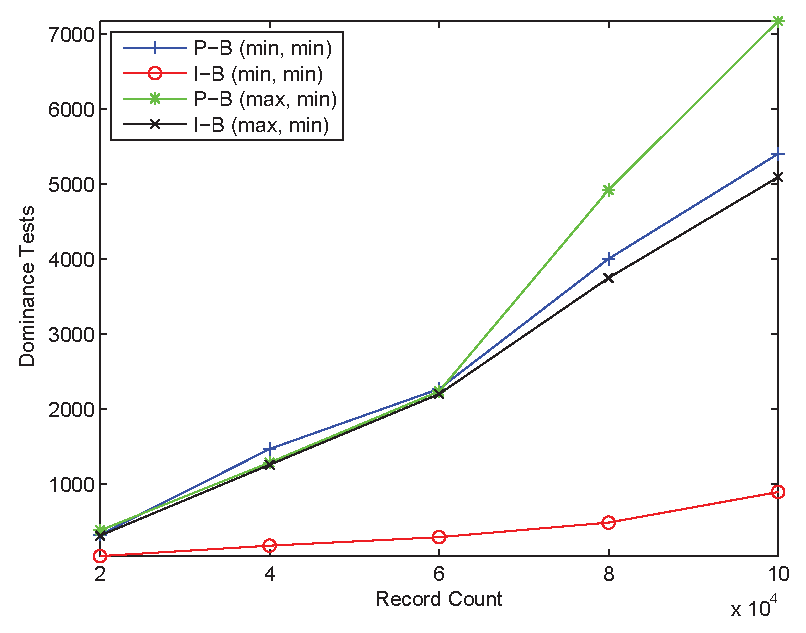
\includegraphics[width=1.6in]{Figures/exp/dt_rc_minmin_maxmin.eps}
    %\end{minipage}
    }
  \subfigure[\small (min, max) and (max, max)]{
    \label{fig:dt_rc_b}
    %\begin{minipage}[h!]{0.5\textwidth}
      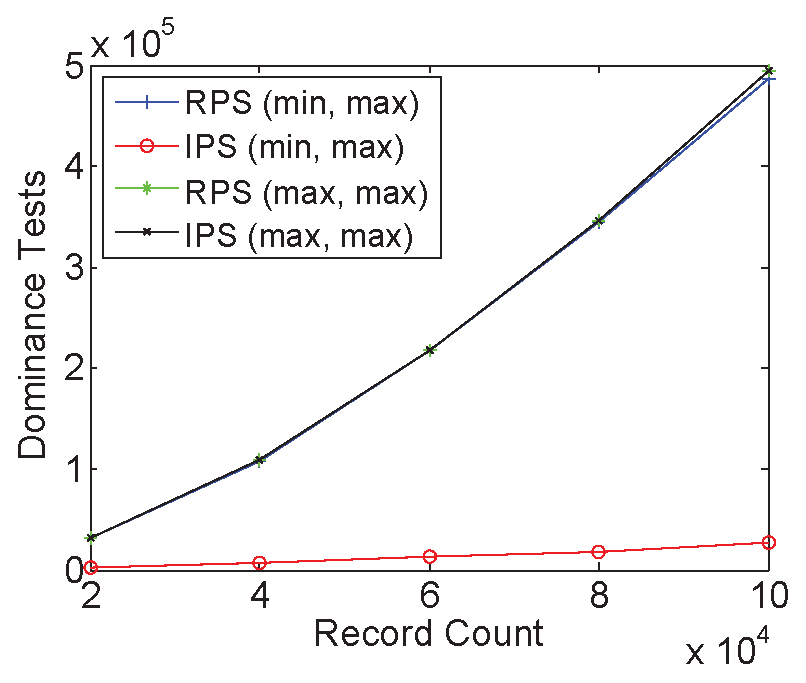
\includegraphics[width=1.6in]{Figures/exp/dt_rc_minmax_maxmax.eps}
    %\end{minipage}
    }
  \caption{\small Dominance Tests vs. Record Count. d = 2, b = 10,
  Data = uniformed}
  \label{fig:dt_rc}
\end{figure}


%%
% Dominance Test vs. Dimensions
%%
\begin{figure}
  \centering
  \subfigure[\small All Min and All Max. Data = uniformed]{
    \label{fig:dt_dim_a}
    %\begin{minipage}[h!]{0.5\textwidth}
      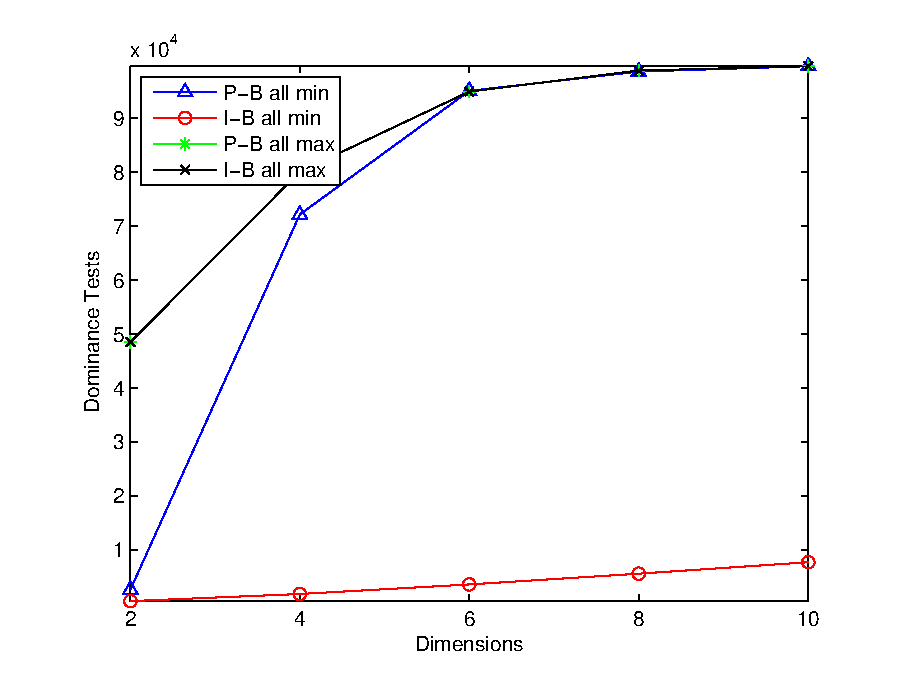
\includegraphics[width=1.6in]{Figures/exp/dt_dim_allmin_allmax.eps}
    %\end{minipage}
    }
  \subfigure[\small Mixed Data Types]{
    \label{fig:dt_dim_b}
    %\begin{minipage}[h!]{0.5\textwidth}
      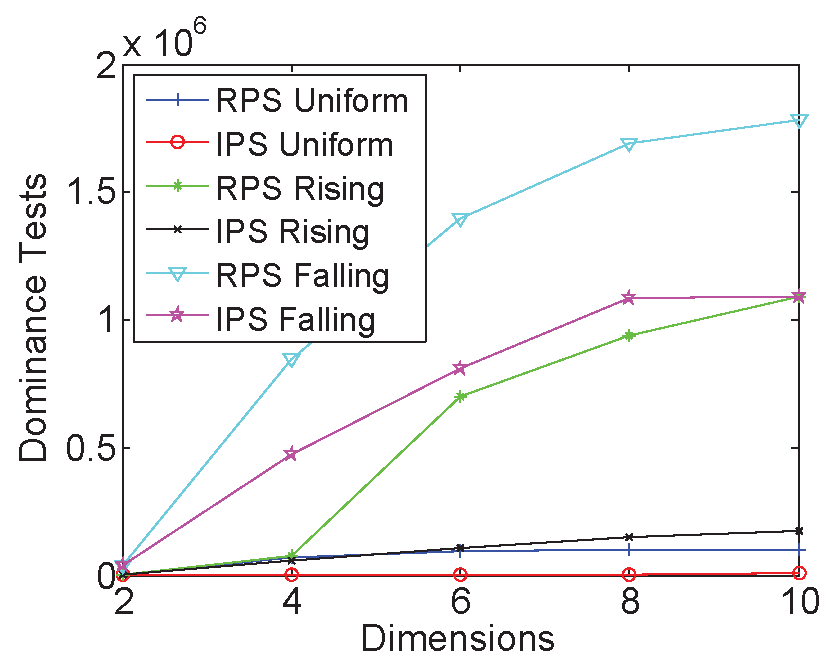
\includegraphics[width=1.6in]{Figures/exp/dt_dim_mixdata_rc10000.eps}
    %\end{minipage}
    }
  \caption{\small Dominance Tests vs. Dimensions. rc = 10000, b = 10}
  \label{fig:dt_dim}
\end{figure}


\subsection{Tuning Time}\label{sec:exp_tuning_time}

As discussed in section~\ref{sec:wireless_broadcast}, tuning time is total
amount of data the client has to download to fulfill a skyline query and
it is measured in bytes. The experiment simulates the server creating the
DFDI broadcast program. Tuning time is found by simulating a client evaluating
a skyline query from the beginning of the cycle.

Figure~\ref{fig:tt_rec} illustrates tuning time versus increasing record count
for all combinations of min and max attribute for 2-dimensional data. In
all cases, the Index-Based (I-P) pruning strategy performs several factors
better than Point-Based (P-B) pruning strategies.

Figure~\ref{fig:tt_dim} illustrates the simulation result for tuning time with
increasing data dimension. The experiments are run with record count (rc) of
10000, and branching factor (b) of index tree of 10.
Although the number of record stays the same, each additional dimension or
data attribute of the data-set adds space complexity to the data-set. With
increasing increasing dimensionality, the cycle length also increases, so
tuning time.

%%
% Tuning Time vs. Record Count
%%
\begin{figure}
  \centering
  \subfigure[\small (min, min) and (max, max)]{
    \label{fig:tt_rec_a}
    %\begin{minipage}[h!]{0.5\textwidth}
      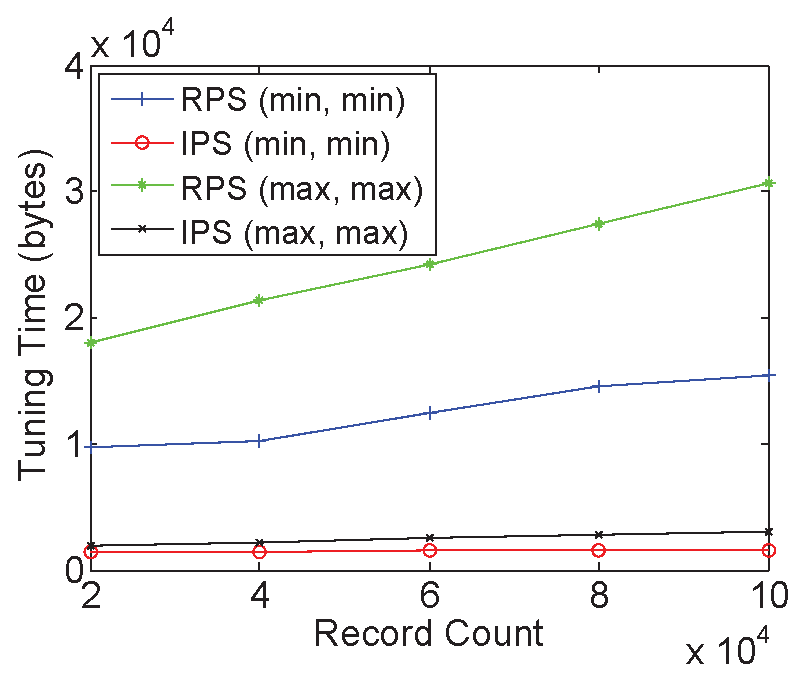
\includegraphics[width=1.6in]{Figures/exp/tt_rc_minmin_maxmax.eps}
    %\end{minipage}
    }
  \subfigure[\small (min, max) and (max, min)]{
    \label{fig:tt_rec_b}
    %\begin{minipage}[h!]{0.5\textwidth}
      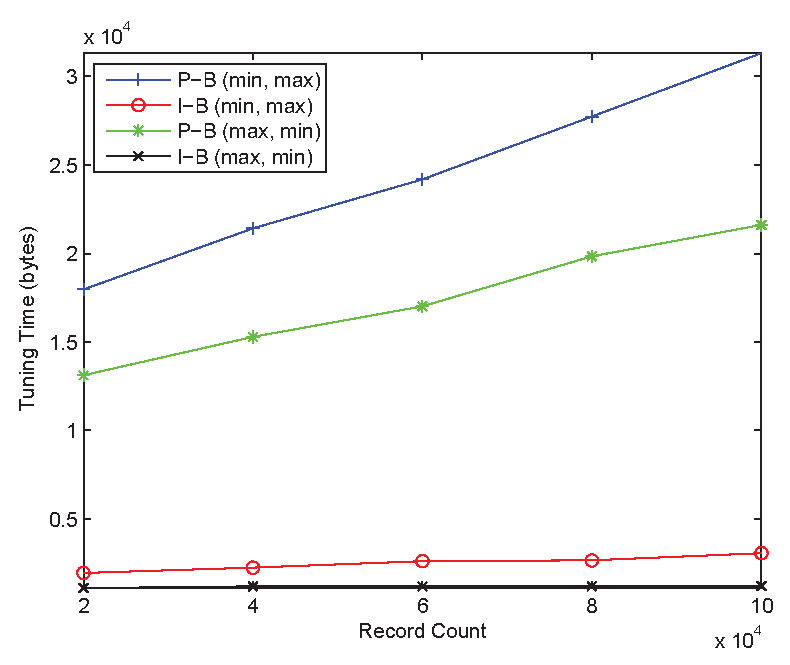
\includegraphics[width=1.6in]{Figures/exp/tt_rc_minmax_maxmin.eps}
    %\end{minipage}
    }
  \caption{\small Tuning Time vs. Record Count. d = 2, b = 10}
  \label{fig:tt_rec}
\end{figure}

%%
% Tuning Time vs. Dimension
%%
\begin{figure}
  \centering
  \subfigure[\small All Min and All Max]{
    \label{fig:tt_dim_a}
    %\begin{minipage}[h!]{0.5\textwidth}
      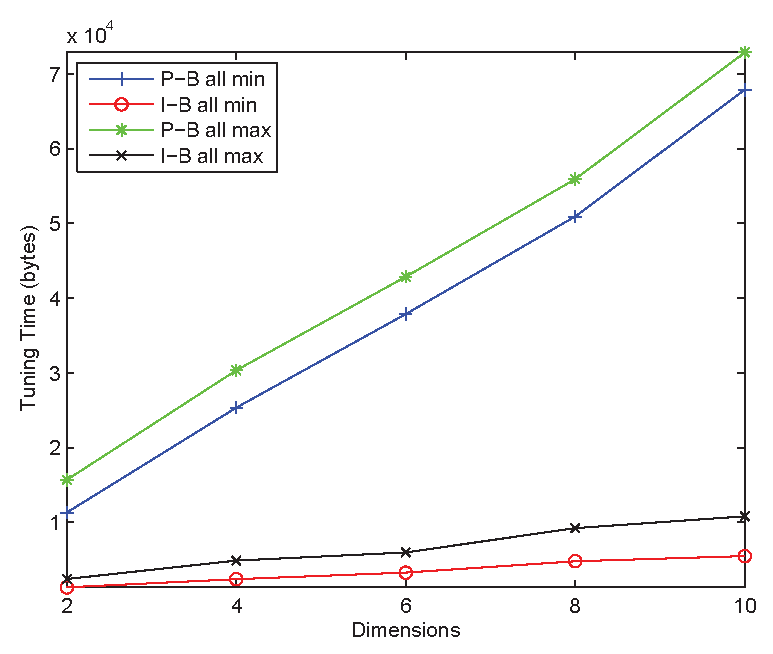
\includegraphics[width=1.6in]{Figures/exp/tt_dim_allmin_allmax_mod.eps}
    %\end{minipage}
    }
  \subfigure[\small Mixed Data Types]{
    \label{fig:tt_dim_b}
    %\begin{minipage}[h!]{0.5\textwidth}
      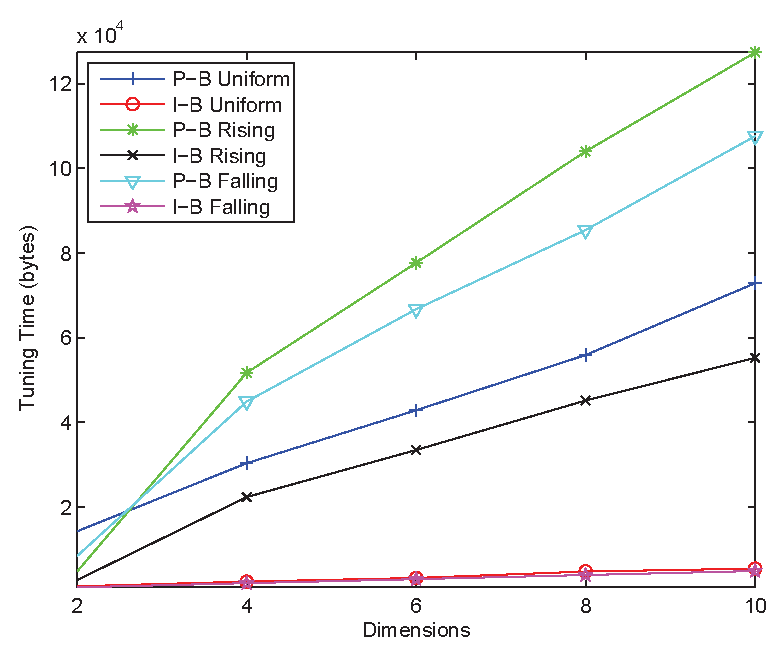
\includegraphics[width=1.6in]{Figures/exp/tt_dim_mixdata_rc10000.eps}
    %\end{minipage}
    }
  \caption{\small Tuning Time vs. Dimensionality. rc = 10000, b = 10}
  \label{fig:tt_dim}
\end{figure}

%%
% Index Percentage
%%
\begin{figure}
  \centering
  \subfigure[\small IP vs. Record Count]{
    \label{fig:ip_rc}
    %\begin{minipage}[h!]{0.5\textwidth}
      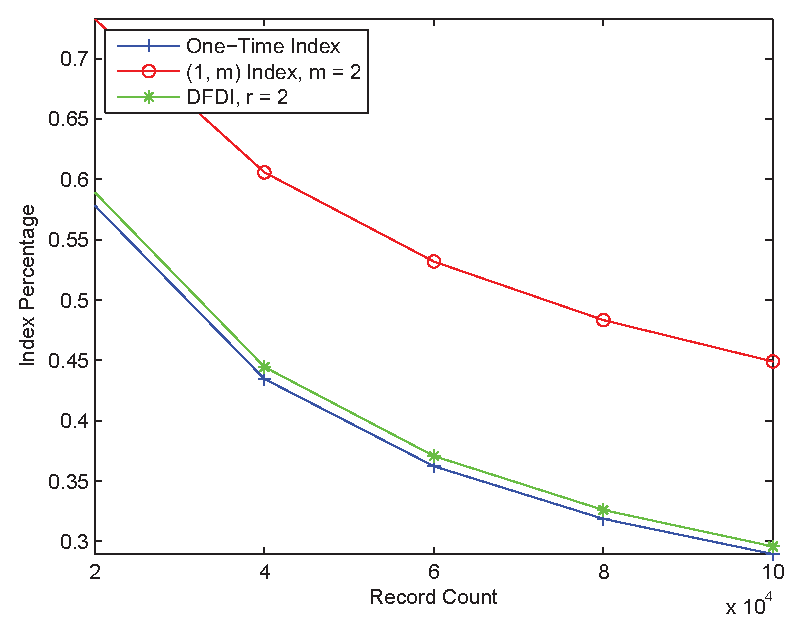
\includegraphics[width=1.6in]{Figures/exp/ip_rc.eps}
    %\end{minipage}
    }
  \subfigure[\small IP vs. Dimensionality]{
    \label{fig:ip_dim}
    %\begin{minipage}[h!]{0.5\textwidth}
      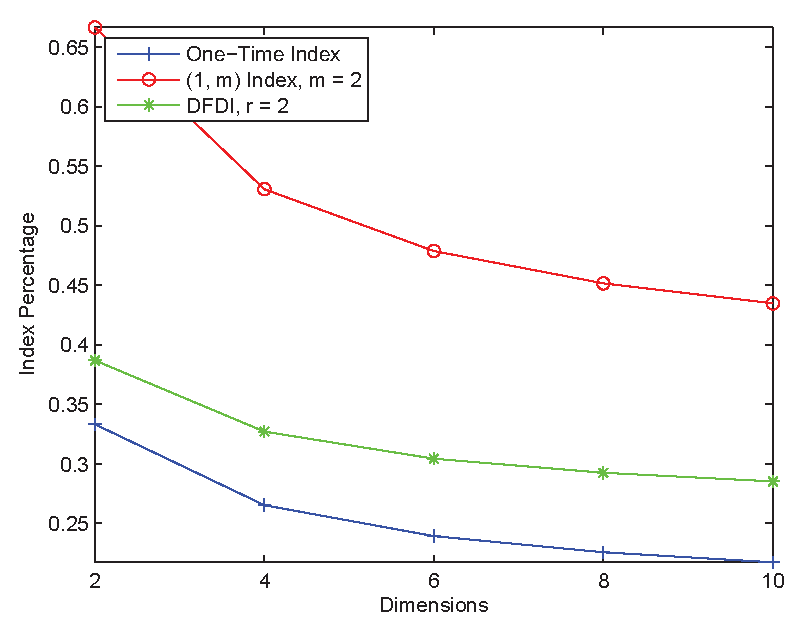
\includegraphics[width=1.6in]{Figures/exp/ip_dim.eps}
    %\end{minipage}
    }
  \caption{\small Index Percentage. b = 10}
  \label{fig:ip}
\end{figure}


\subsection{Index Percentage}

Index percentage measures the efficiency of the DFDI broadcast program
allocation technique under increasing record count and increasing data
dimension. Index percentage is defined in
section~\ref{sec:wireless_broadcast}.

Figure~\ref{fig:ip_rc} shows index percentage versus increasing record
count. For the DFDI, the simulation is run with replication level of 2,
which means the root and the first level below the root are replicated.
For the (1, m) index, m = 2, meaning the complete index is duplicated
2 times in the broadcast cycle.
The figure shows that the overhead of the index is high when the
number of record is low, but the overhead flattens as the number of
records grow. The one-time index is the baseline and as expected has
the lowest index percentage. Although DFDI replicated the index for
2 levels, its index percentage is only slightly (16\%) higher than
one-time index. This shows DFDI is efficient in terms of space
overhead. Whereas the (1, m) index has far worse overhead for only
2 duplications.

Figure~\ref{fig:ip_dim} shows index percentage over increasing data
dimension. The experiment is conducted with 10000 records and branching
factor of 10. As the data size grows with the number of dimensions, the
index is only slightly affected by the growth. The size of index grows
because of the index needs extra information to index the extra
dimensions, but the tree height is largely unaffected; thus gives the
falling of index percentage with growing dimension.

%Simulate 3 algorithms:
%\begin{enumerate}
%\item R-Tree one-time index \item R-Tree DFDI \item Grid R-Tree
%DFDI
%\end{enumerate}

%Measurements:
%\begin{enumerate}
%\item Index percentage (with variable branching factor) \item
%Tuning time (with variable branching factor) \item Dominance tests
%(with variable branching factor)
%\end{enumerate} 